
\section*{Comunicazioni digitali}


\begin{adjustwidth*}{-2.3cm}{-2cm}
    \begin{center}
        \begin{tikzpicture}[>=Stealth, block/.style={draw, rectangle}, scale=0.85]
            % Blocks
            \tikzstyle{block} = [rectangle, draw, text centered, minimum height=4em, align=center]

            \node[block] (mod) {Modulatore \\ numerico};
            \node[block, right=1cm of mod] (channel) {Canale di \\ comunicazione};
            \node[block, right=1cm of channel] (demod) {Demodulatore \\ numerico};

            % Nodes for connecting lines
            \coordinate[left=2cm of mod] (input);
            \coordinate[right=2cm of demod] (output);

            % Lines
            \draw[->] (input) -- node[above] {$m_s[n]$} (mod);
            \draw[->] (mod) -- node[above] {$s(t)$} (channel);
            \draw[->] (channel) -- node[above] {$r(t)$} (demod);
            \draw[->] (demod) -- node[above] {$\hat{m}_s[n]$} (output);

            % Dashed box
            \begin{scope}
                \draw[dashed, red] ($(mod.north west)+(-0.5,0.5)$) rectangle ($(demod.south east)+(0.5,-0.5)$);
            \end{scope}

            % Annotations
            \node[align=center, red, above right= -1cm and -6cm of demod.south east] (channel-label) {Canale numerico};

            % Circles
            \draw (input) ++(-0.5cm,0) circle (0.5cm) node {$S$};
            \draw (output) ++(0.5cm,0) circle (0.5cm) node {$D$};
        \end{tikzpicture}
    \end{center}
\end{adjustwidth*}




In una comunicazione digitale l'informazione è codificata in sequenze di bit. Se rappresentassimo ogni bit come un funzione delta otterremmo un treno di delta:
\[
    \sum_{k=-\infty}^{+\infty} d_k \delta(t - kT_b)
\]
che occupa però una banda infinita.

La modulazione PAM consiste nell'effettuare il mapping dei bit ed effettuare un filtraggio con un filtro passa basso avente risposta all'impulso \( g_T(t) \), ottenendo:
\[ s_{PAM}(t) \coloneqq \sum_{k=-\infty}^{+\infty} a_k\cdot g_T(t - kT_s) \]

Una sequenza di bit può essere trattata come una variabile aleatoria con distribuzione uniforme:
\[
    P(d_k = 0) = P(d_k = 1) = \frac{1}{2} 
\]
\[
    \mathbb{E}\{d_k\} = 0\cdot P(d_k = 0) + 1\cdot P(d_k = 1) = \frac{1}{2}
\]


% \begin{center}
%     \begin{tikzpicture}
%         \begin{axis}[
%                 title={\( (M=4) \)},
%                 xlabel={},
%                 ylabel={},
%                 xmin=-5, xmax=5,
%                 ymin=-4, ymax=4,
%                 grid=both,
%                 grid style={line width=.1pt, draw=gray!10},
%                 major grid style={line width=.2pt,draw=gray!50},
%                 minor tick num=5,
%                 axis lines=middle,
%                 minor tick style={draw=none},
%                 xtick={-3, -1, 1, 3},
%                 ytick=\empty,
%             ]
% 
%             \addplot+[only marks] coordinates {
%                     (-3, 0)
%                     (-1, 0)
%                     (1, 0)
%                     (3, 0)
%                 };
%         \end{axis}
%     \end{tikzpicture}
% \end{center}
\[
    E_{s_{PAM}}(i) = \int_{-\infty}^{+\infty} s_{PAM, i}^2(t) \, dt =  \int_{-\infty}^{+\infty} \alpha_i^2 \cdot g_T^2(t - kT_s) \, dt = \int_{-\infty}^{+\infty} (2i - 1 - M)^2 g_T^2(t) \, dt = (2i - 1 - M)^2 E_{g_T}
\]

Scegliendo una mappatura simmetrica dei bit, possiamo trasmettere simboli con media nulla e quindi con energia a media nulla:
\[
    a_i = 
    \begin{cases}
        -1 & \text{se } d_k = 0 \\
        1 & \text{se } d_k = 1
    \end{cases}
\]
Per \( M \) pari si ha \( A_s = \{ \pm 1, \pm 3, \ldots, \pm (M-1) \} \)

Per \( M \) dispari si ha \( A_s = \{ 0, \pm 2, \pm 4, \ldots, \pm (M-1) \} \)


Gli \( M \) valori \( (M \geq 2) \) che costituiscono l'alfabeto \( A_s = \{ \alpha_1, \alpha_2, \ldots, \alpha_M \} \) sono definiti come:
\[ \alpha_i = 2i - 1 - M, \quad i = 1, 2, \ldots, M \]




\subsection*{Proprietà derivate della M-PAM}
\begin{enumerate}
    \item Il valor medio di \( s(t) \) è zero per ogni \( t \):
          \begin{equation*}
              \mathbb{E}\left[ s(t) \right] = 0 \quad \forall t
          \end{equation*}
          \begin{equation*}
              \mathbb{E} \left[ \sum_{k=-\infty}^{+\infty} a[k] \ p(t-kT_s) \right] = \sum_{k=-\infty}^{+\infty} \mathbb{E}\left[a[k]\right]\ p(t-kT_s) = 0
          \end{equation*}
          \begin{equation*}
              \mathbb{E}\left[a[k]\right] = \frac{1}{M} \sum_{i=1}^{M} \alpha_i \mathbb{P}\{\alpha_i\} = \frac{1}{M} \sum_{i=1}^{M} (2i - 1 - M)
          \end{equation*}
          \begin{equation*}
              = \frac{2}{M} \sum_{i=1}^{M} i - 1 - M = \frac{2}{M} \frac{M(M+1)}{2} - (M+1) = 0
          \end{equation*}

    \item La densità spettrale di potenza invece è:
          \begin{equation*}
              S_s(f) = \frac{1}{T_s} S_a(f) \ |G_T(f)|^2
          \end{equation*}
          \begin{equation*}
              \text{dove } \sigma_a^2 = \mathbb{E}\left[ a\left[k\right]^2 \right] = \frac{(M-1)(M+1)}{3}
          \end{equation*}
\end{enumerate}

\[
    R_s(t,\tau) = \mathbb{E}[s(t) \ s^*(t-\tau)]
\]
\[
    = \mathbb{E} \left[ \sum_{n=-\infty}^{+\infty} a\left[n\right] g_T(t - nT_s) \sum_{k=-\infty}^{+\infty} a^*\left[k\right] g_T^*(t - \tau - kT_s) \right]
\]
\[
    = \sum_{n=-\infty}^{+\infty} \sum_{k=-\infty}^{+\infty} \mathbb{E}[a\left[n\right] a^*\left[k\right]] \cdot g_T(t - nT_s) \cdot g_T^*(t - \tau - kT_s)
\]
\[
    = \sum_{n=-\infty}^{+\infty} \sum_{k=-\infty}^{+\infty} R_a\left[n-k\right] \cdot g_T(t - nT_s) \cdot g_T^*(t - \tau - kT_s)
\]

Imponendo \( n-k = m \) abbiamo che \( k = n-m \), quindi:

\[
    = \sum_{m=-\infty}^{+\infty} R_a[m] \sum_{n=-\infty}^{+\infty} g_T(t - nT_s) \cdot g_T^*(t - \tau - nT_s + mT_s)
\]

\paragraph*{Autocorrelazione media}

La funzione di autocorrelazione media \( \overline{R}_s(\tau) \) è:
\begin{align*}
    \overline{R}_s(\tau) & = \lim_{T\to\infty} \frac{1}{T} \int_{-\frac{T}{2}}^{\frac{T}{2}} R_s(t, \tau) dt                                                                   \\
    \overline{R}_s(\tau) & = \frac{1}{T_0} \int_{-\frac{T_0}{2}}^{\frac{T_0}{2}} R_s(t,\tau)dt \quad \text{se} \quad R_s(t,\tau) \quad \text{è periodico in} t           \\
    \overline{R}_s(\tau) & = \sum_{m=-\infty}^{\infty} R_a[m] \frac{1}{T_s} \sum_{n=-\infty}^{\infty} \int_{-\frac{T_s}{2}}^{\frac{T_s}{2}} g_T(t-nT_s)g_T^*(t-\tau-nT_s+mT_s)dt   \\
                         & = \sum_{m=-\infty}^{\infty} R_a[m] \frac{1}{T_s} \sum_{n=-\infty}^{\infty}\int_{-\frac{T_s}{2}+nT_s}^{\frac{T_s}{2}+nT_s} g_T(t')g_T^*(t'-\tau+mT_s)dt' \\
                         & = \sum_{m=-\infty}^{\infty} R_a[m] \frac{1}{T_s} \int_{-\infty}^{\infty} g_T(t')g_T^*(t'-\tau+mT_s)dt'                                                  \\
                         & = \sum_{m=-\infty}^{\infty} R_a[m] \frac{1}{T_s} \int_{-\infty}^{\infty} G_T(f)[G_T(f)e^{-j2\pi f\tau}e^{j2\pi fmT_s}]^*df                              \\
                         & = \int_{-\infty}^{\infty} G_T(f)G_T^*(f)\frac{1}{T_s} \sum_{m=-\infty}^{\infty} R_a[m] e^{-j2\pi fmT_s}e^{j2\pi f\tau}df                                \\
                         & = \frac{1}{T_s} \int_{-\infty}^{\infty} |G_T(f)|^2 S_a(f)e^{j2\pi f\tau}df
\end{align*}


\[
    \overline{R}_s(\tau) = \frac{1}{T_s} TCF^{-1} \left[ |G_T(f)|^2 S_a(f) \right]
\]
\[
    \Rightarrow S_s(f) = \frac{1}{T_s} S_a(f) |G_T(f)|^2
\]

Nel caso in cui:
\begin{enumerate}
    \item $\mathbb{E} [ a[n] ] = 0$
    \item $R_a[m] = \sigma_a^2 \delta[m]$
\end{enumerate}

Si ha che:
\[
    S_s(f) = \frac{\sigma_a^2}{T_s} |G_T(f)|^2
\]

In questo caso la $B_T$ coincide con quella del sagomatore $G_T(f)$.

Calcolo di $\sigma_a^2$:
\[
    \sigma_a^2 = \mathbb{E} \left[ (a - \mu_a)^2 \right] = \int_{-\infty}^{\infty} (a - \mu_a)^2 f_a(a) da
\]
\[
    = \frac{1}{M} \sum_{i=1}^{M} (2i - 1 - M)^2
\]
\[
    = \frac{1}{M} \left[ 2 \sum_{i=1}^{M} i^2 + (1+M)^2 M - 4(1+M) \sum_{i=1}^{M} i \right]
\]

Sfruttando i seguenti risultati noti:
\[
    \sum_{i=1}^{n} i^2 = \frac{n(n+1)(2n+1)}{6}, \quad \sum_{i=1}^{n} i = \frac{n(n+1)}{2}
\]

Si ottiene:
\[
    \sigma_a^2 = \frac{M^2 - 1}{3}
\]

\[
    P_s = \frac{\sigma_a^2 E_{g_T}}{T_s} = \frac{M^2 - 1}{3} \frac{E_{g_T}}{T_s}
\]


Come sarà dimostrato più avanti, $R_s \propto B$, dove $B$ è la banda del segnale $s_{PAM}(t)$. 
Per $R_s$ valgono le seguenti equivalenze:
\[
    R_s = \frac{1}{T_s} = \frac{1}{mT_s} = \frac{R_b}{m} = \frac{R_b}{\log_2 M}
\]

Dove $R_b$ è il bit rate.




\paragraph*{Efficienza Spettrale di una M-PAM} TODO
\[
    \beta = \frac{R_b}{B_T} = \frac{\log_2 M}{T_s B_{g_T}}
\]
essendo \( B_T = B_{g_T} \),

L'efficienza spettrale aumenta con l'aumentare del numero di livelli. Sfortunatamente, come verrà dimostrato più avanti, l'efficienza in potenza diminuisce all'aumentare di \( M \).

\begin{center}
    \begin{tikzpicture}[
            block/.style={rectangle, draw, minimum height=1cm, minimum width=2cm},
            node distance=1cm,
            auto
        ]
        \node[draw, circle] (source)  {S};
        \node[block, right= of source] (interpolatore) {PAM tx};
        \node[left=of interpolatore] (tmp) {};
        \node[block, right= of interpolatore] (chan) {$h(t)$};

        \node[draw, circle, right= of chan] (plus)  {\(+\)};
        \node[below=of plus, inner sep=0pt, minimum size=0pt] (n) {};
        \node[block, right=of plus] (sampler) {PAM rx};
        \node[circle, draw, right=of sampler] (dest) {D};
        
        \draw[->] (source) -- (interpolatore) node[midway,above] {$d_k$};
        \draw[->] (interpolatore) -- (chan) node[midway,above] {$\tilde{s}(t)$};
        \draw[->] (chan) -- (plus) node[midway,above] {$y(t)$};
        \draw[->] (plus) -- (sampler) node[midway,above] {$r(t)$};
        \draw[->] (n) -- (plus) node[midway, right] {$w(t)$};
        \draw[->] (sampler) -- (dest) node[midway,above] {$\hat{d}_k$};
    \end{tikzpicture}
\end{center}




Il canale di comunicazione è generalmente modella come un sistema LTI, caratterizzato da una risposta impusliva $h(t)$ e da un rumore additivo $w(t)$.
Nel caso ideale $h(t) = \delta (t)$.
Il rumore aggiunto al segnale si modella come rumore bianco gaussiano a potenza spettrale costante $N_0/2$, col quale si modella il disturbo proveniente dalle radiazioni solari, dalle radiazioni del big bang e del rumore dei dispositivi.
Il ricevitore è composto da 3 componenti principali:
\begin{enumerate}
    \item \textbf{Filtro passa basso}, che filtra il segnale ricevuto per eliminare le frequenze superiori a $B_T$.
    \item \textbf{Campionatore}, che campiona il segnale filtrato con rate $1/T_s$. 
    \item \textbf{Decisore}, che associa ad ogni campione un simbolo appartenente alla costellazione.
\end{enumerate}
Il segnale ricevuto è il seguente:
\[
    r(t) = s(t) \ast h(t) + w(t)
\]

mentre il segnale filtrato è:
\[
    x(t) = r(t) \ast g_R(t) = \sum_{k=-\infty}^{+\infty} a_k g(t - kT_s) + n(t)
\]
dove $g(t) = g_T(t) \ast h(t) \ast g_R(t)$ e $n(t) = w(t) \ast g_R(t)$. La densità spettrale di energia del rumore diventa:
\[
    S_n(f) = S_w(f) |G_R(f)|^2
\]



\subsection*{Interferenza intersimbolica (ISI)}
\noindent
\begin{minipage}{.5\textwidth}
    \centering
    \textbf{Assenza di ISI:}
    \[
        x[k] = f(a[k])
    \]
    \\
\end{minipage}%
\begin{minipage}{.5\textwidth}
    \centering
    \textbf{Presenza di ISI:}
    \[
        x[k] = f(\dots, a[k-1], a[k], a[k+1], \dots)
    \]
    \\
\end{minipage}


Il risultato è che il campione estratto al ricevitore dal segnale ricevuto al $k$-esimo istante non dipende solo dal $k$-esimo simbolo.

\begin{center}
    \begin{tikzpicture}[
            block/.style={rectangle, draw, minimum height=1cm, minimum width=2.5cm},
            node distance=1cm and 2cm,
            auto
        ]

        \node[block] (filter) {$g_R(t)$};
        \node[left=of filter] (channel) {};
        \node[right=of filter] (sampler) {};

        \draw[->] (channel) -- (filter) node[midway,above] {$r(t)$};

        \draw ([xshift=0]filter.east) -- ([xshift=1cm]filter.east) node[midway,above] {$x(t)$};
        \draw ([xshift=1cm]filter.east) -- ([xshift=1.5cm,yshift=0.5cm]filter.east) node[midway,below, yshift=-0.2cm] {$T_s$};

        \draw[->] ([xshift=1.5cm,yshift=0cm]filter.east) -- ++(1.5cm,0) node[midway,above] {$x[k]$};


    \end{tikzpicture}
\end{center}

dove:
\[
    x(t) = r(t) \ast g_R(t) = \sum_{k=-\infty}^{+\infty} a_k g(t - kT_s) + n(t)
\]
campionato in $t = mT_s$ si ha:
\[
        x(mT_s) = x[m] = \sum_{k=-\infty}^{+\infty} a_k g(mT_s - kT_s) + n(mT_s) = \sum_{k=-\infty}^{+\infty} a_k g[m-k] + n[m] \\ 
 \]
\[
        = a_m g(0) + \sum_{\substack{k \neq m, k=-\infty}}^{+\infty} a_k g[m-k] + n[m]
\]



Un canale con banda \( B_c \) in generale introduce ISI. Ci sono due aspetti di cui ci occuperemo:

\begin{enumerate}
    \item Determinazione del \( T_s \) minimo che può essere adottato al fine di ottenere una sequenza campionata priva di ISI.
    \item Determinare le condizioni sotto le quali è possibile trasmettere un segnale M-PAM attraverso un canale non ideale in modo che non vi sia ISI nella sequenza campionata.
\end{enumerate}

Nel risolvere i due problemi riterremo \( h(t) \) fissata, e \( g_T(t) \) e \( g_R(t) \) variabili, in quanto determinabili dal progettista.

Un approccio non perseguibileconsiste nel trasmettere impulsi di durata finita e quindi con banda illimitata. Questo è in contrasto con la limitatezza messa a disposizione dal canale di trasmissione \( (B_c < \infty) \).

\(\Rightarrow\) Gli impulsi \( g_T(t) \) devono avere durata infinita.

\paragraph{Criterio di Nyquist}*{Primo criterio di Nyquist per la trasmissione priva di ISI}

\[ g(kT_s) =
    \begin{cases}
        1, & \text{se } k=0      \\
        0, & \text{se } k \neq 0
    \end{cases}
    \quad \text{(Dominio del tempo)}
\]

\[ \sum_{k=-\infty}^{+\infty} G\left(f-\frac{k}{T_s}\right) = T_s \quad \text{(Dominio della frequenza)} \]




\paragraph*{Dimostrazione}
Il criterio di Nyquist nel dominio del tempo garantisce l'assenza di ISI in quanto
\[ x[k] = a[k] \cdot g(0) + \sum_{\substack{i=-\infty \\ i \neq k}}^{+\infty} a[i] \cdot g[i-k] = a[k] \cdot g(0) \]
dove il secondo termine è nullo e non vi è ISI se \( g[k] = \delta[k] \).

La relazione in frequenza si ottiene come trasformazione
\[ g[k] = \delta[k] \quad \Longleftrightarrow \quad \overline{G}(f) = 1 \]
\[ \overline{G}(f) = \frac{1}{T_s} \sum_{k=-\infty}^{+\infty} G\left(f - \frac{k}{T_s}\right) = 1 \]
\[ \sum_{k=-\infty}^{+\infty} G\left(f - \frac{k}{T_s}\right) = T_s \]

\paragraph*{Trasmissione priva di ISI}
Supponiamo sia assegnato un canale a banda rigorosamente limitata con banda \( B_c \).
\[ H(f) = 0 \quad \text{per} \quad |f| > B_c \]
e supponiamo che \( B_T = B_c \), ovvero che il segnale trasmesso occupa tutta la banda messa a disposizione dal canale.
Allora si verificano le seguenti:
\begin{enumerate}
    \item Non è possibile in alcun modo eliminare l'ISI quando \( T_s < \frac{1}{2B_c} \).


          \paragraph*{Dimostrazione:}

          Quando \( T_s < \frac{1}{2B_c} \)

          \begin{tikzpicture}[scale=0.5]
              \draw[->] (-15,0) -- (15,0) node[right] {\( f \)};
              \draw[->] (0,-1) -- (0,7) node[above] {\( \overline{G}(f) \)};

              % Triangles
              \draw (-11,0) -- (-8,3) -- (-5,0);
              \draw[dashed, red] (-5,-1) -- (-5,4);
              \draw[dashed, red] (-3,-1) -- (-3,4);
              \draw (-3,0) -- (0,3) -- (3,0);
              \draw[dashed, red] (3,-1) -- (3,4);
              \draw[dashed, red] (5,-1) -- (5,4);
              \draw (5,0) -- (8,3) -- (11,0);

              \node at (-12,1.5) {\( \cdots \)};
              \node at (12,1.5) {\( \cdots \)};
          \end{tikzpicture}

          Esistono degli intervalli di frequenza dove \( \overline{H}(f) = 0 \) per cui non può mai accadere che \( \overline{H}(f) = 1 \) \( \forall f \)

          \bigskip

    \item Il più piccolo valore di \( T_s \) che permette di eliminare l'\( ISI \) è

          \( T_s^{(min)} = \frac{1}{2B_c} \)

          \bigskip

          \( f_s^{(max)}\) = \( \frac{1}{T_s^{(min)}} = 2B_c = f_N \) \quad (frequenza di Nyquist)

          \bigskip

          \begin{tikzpicture}[scale=0.5]
              \draw[->] (-15,0) -- (15,0) node[right] {\( f \)};
              \draw[->] (0,-1) -- (0,7) node[above] {\( \overline{G}(f) \)};

              % Triangles
              \draw (-9,0) -- (-6,3) -- (-3,0);
              \draw (-3,0) -- (0,3) -- (3,0);
              \draw (3,0) -- (6,3) -- (9,0);

              \node at (-10,1.5) {\( \cdots \)};
              \node at (10,1.5) {\( \cdots \)};
              \
          \end{tikzpicture}

          Non esistono intervalli di frequenza dove \( \overline{G}(f) = 0 \)

          \bigskip

    \item Nel caso valga la condizione \( T_s = \frac{1}{2B_c} \), allora l'unica funzione di trasferimento che permette di eliminare completamente l'ISI è

          \[ G(f) = \frac{1}{2B_c} \text{rect}\left(\frac{f}{2B_c}\right) \quad \Leftrightarrow \quad g(t) = \text{sinc}(2B_c t) \]

          \paragraph*{Dimostrazione:}

          \begin{center}

              \begin{tikzpicture}[scale=1]
                  \begin{axis}[
                          axis lines=middle,
                          xlabel={$f$},
                          ylabel={$G(f)$},
                          xtick={-4, -2, 2, 4},
                          xticklabels={$-2B_c$, $-B_c$, $B_c$, $2B_c$},
                          ytick={100},
                          yticklabels={},
                          ymin=-0.2, ymax=2,
                          xmin=-8, xmax=8,
                          xmajorgrids=false,
                          ymajorgrids=false,
                          clip=false
                      ]

                      \draw [thick] (axis cs:-2,0) rectangle (axis cs:2,0.4);

                      \node [red]at (axis cs:7,0.6) {$\sum_{k=-\infty}^{\infty} G(f - \frac{k}{T_s})$};

                      \draw [dashed, red] (axis cs:-6,0.4) -- (axis cs:-6,0);
                      \draw [dashed, red] (axis cs:-8,0.4) -- (axis cs:-2,0.4);
                      \draw [dashed, red] (axis cs:2,0.4) -- (axis cs:8,0.4);
                      \draw [dashed, red] (axis cs:6,0.4) -- (axis cs:6,0);
                  \end{axis}
                  \
              \end{tikzpicture}
          \end{center}

          Si nota anche che la funzione $\text{sinc}(2Bt)$ si annulla quando $t = \frac{k}{2B}$ con $k \neq 0$ per cui
          \[
              g(kT_s) = \text{sinc} \left(2B_c\cdot\frac{k}{2B_c}\right) = \text{sinc}(k) = 
              \begin{cases}
                  1 & \text{se } k=0    \\
                  0 & \text{se } k\neq0
              \end{cases}
          \]
\end{enumerate}


\textbf{Limiti di applicabilità della funzione di trasferimento rettangolare:}

\begin{enumerate}
    \item Realizzabilità di una funzione di trasferimento rettangolare: risposte in frequenza ideali come quella rettangolare non sono fisicamente realizzabili (Criterio di Paley-Wiener).
    \item Piccoli errori di campionamento provocano un ISI molto grande poiché la funzione $\text{sinc}(2B_ct)$ decresce molto lentamente.
\end{enumerate}

Un errore è nel campionatore induce un ISI grande in quanto si sommano molte contributi!




\begin{figure}[ht]
    \centering
    \begin{center}
        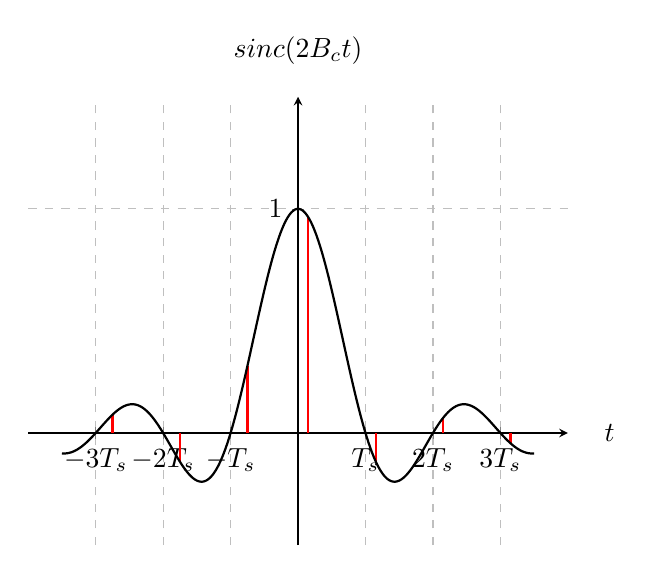
\begin{tikzpicture}
            \begin{axis}[
                    axis lines=middle,
                    xlabel={$t$},
                    ylabel={$\text{sinc}(2B_c t)$},
                    xtick={-3, -2, -1, 0, 1, 2, 3},
                    xticklabels={$-3T_s$, $-2T_s$, $-T_s$, $0$, $T_s$, $2T_s$, $3T_s$},
                    ytick={1},
                    ymin=-0.5, ymax=1.5,
                    xmin=-4, xmax=4,
                    every axis x label/.style={at={(ticklabel* cs:1.05)}, anchor=west,},
                    every axis y label/.style={at={(ticklabel* cs:1.05)}, anchor=south,},
                    xmajorgrids=true,
                    ymajorgrids=true,
                    grid style=dashed,
                    clip=false,
                    no markers,
                    samples=1000,
                    domain=-3.5:3.5
                ]


                \draw [thick, red] (axis cs:-2.75,0) -- (axis cs:-2.75,0.082);
                \draw [thick, red] (axis cs:-1.75,0) -- (axis cs:-1.75,-0.13);
                \draw [thick, red] (axis cs:-0.75,0) -- (axis cs:-0.75,0.30);

                \draw [thick, red] (axis cs:0.15,0) -- (axis cs:0.15,0.965);

                \draw [thick, red] (axis cs:1.15,0) -- (axis cs:1.15,-0.125);
                \draw [thick, red] (axis cs:2.15,0) -- (axis cs:2.15,0.07);
                \draw [thick, red] (axis cs:3.15,0) -- (axis cs:3.15,-0.045);


                % Define sinc function
                \addplot+[thick, black, smooth, unbounded coords=jump] {sin(deg(pi*x))/(pi*x)};
                \addplot+[thick, black, smooth] coordinates {(0, 1)};

                % Add the red vertical line at t=0

            \end{axis}
        \end{tikzpicture}
    \end{center}
    \caption*{Un errore $\epsilon$ nel campionatore induce un ISI grande in quanto si sommano molti contributi. In rosso l'errore $\epsilon$ del compionatore.}
    %\label{fig:my_label} % Optional, for referencing the figure
\end{figure}



Rilassando la condizione $T_s > \frac{1}{2B_c}$, ovvero ammettendo

\[ T_s > \frac{1}{2B_c} \]

si ottiene il seguente effetto:

\begin{center}

    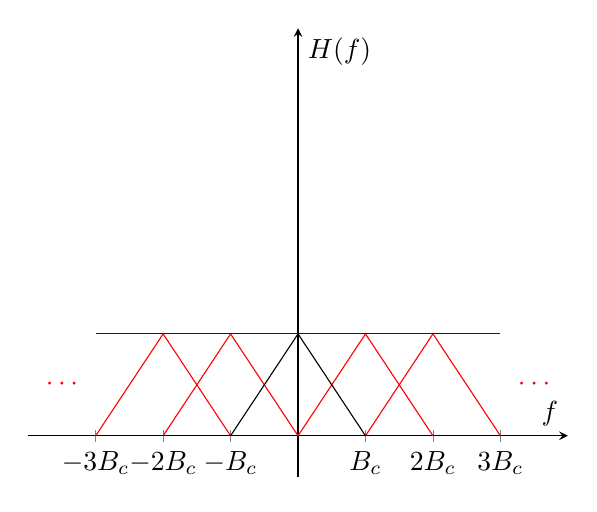
\begin{tikzpicture}[scale=1]
        \begin{axis}[
                axis lines=middle,
                xlabel={$f$},
                ylabel={$H(f)$},
                xtick={-6, -4, -2, 2, 4, 6},
                xticklabels={$-3B_c$, $-2B_c$, $-B_c$, $B_c$, $2B_c$, $3B_c$},
                ytick={100},
                yticklabels={},
                ymin=-0.2, ymax=2,
                xmin=-8, xmax=8,
                %every axis x label/.style={at={(ticklabel* cs:1.05)}, anchor=west,},
                %every axis y label/.style={at={(ticklabel* cs:1.05)}, anchor=south,},
                xmajorgrids=false,
                ymajorgrids=false,
                clip=false
            ]

            \node[red] at (-7,0.25) {\( \cdots \)};

            \draw[red] (-6,0) -- (-4,0.5) -- (-2,0);
            \draw[red] (-4,0) -- (-2,0.5) -- (0,0);

            \draw[red] (0,0) -- (2,0.5) -- (4,0);
            \draw[red] (2,0) -- (4,0.5) -- (6,0);

            \node[red] at (7,0.25) {\( \cdots \)};

            \draw[blue] (-6,0.5) -- (6,0.5);

            \draw (-2,0) -- (0,0.5) -- (2,0);


        \end{axis}
    \end{tikzpicture}
\end{center}

La sovrapposizione permette di definire una classe di infinite funzioni di trasferimento che soddisfano il primo criterio di Nyquist.

In questo caso però $B_c > \frac{1}{2T_s}$, per cui al punto di $T_s$ c'è bisogno di una banda disponibile nel canale che è maggiore di quella che occorre con la funzione di trasferimento rettangolare.

\subsection*{Filtro a coseno rialzato}

% Define the piecewise function
\[ H_{rc}(f) =
    \begin{cases}
        T_s                                                                                                          & \text{if } 0 \leq |f| \leq \frac{1-\alpha}{2T_s}                  \\
        \frac{T_s}{2} \left[ 1 - \sin\left(\frac{\pi T_s}{\alpha} \left( |f| - \frac{1}{2T_s} \right)\right) \right] & \text{if } \frac{1-\alpha}{2T_s} < |f| \leq \frac{1+\alpha}{2T_s} \\
        0                                                                                                            & \text{if } |f| > \frac{1+\alpha}{2T_s}
    \end{cases}
\]

con $0 < \alpha < 1$.

\begin{center}

    \definecolor{myblue}{RGB}{30,144,255}
    \definecolor{myred}{RGB}{178,34,34}
    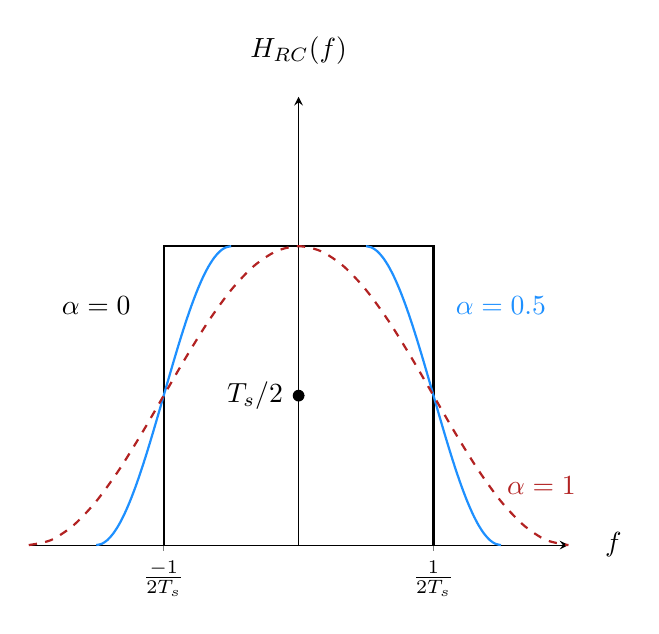
\begin{tikzpicture}
        \begin{axis}[
                axis lines=middle,
                xlabel={$f$},
                ylabel={$H_{RC}(f)$},
                xtick={-0.5, 0.5},
                xticklabels={$\frac{-1}{2T_s}$, $\frac{1}{2T_s}$},
                ytick={0.5},
                yticklabels={$T_s/2$},
                ymin=0, ymax=1.5,
                xmin=-1, xmax=1,
                every axis x label/.style={at={(ticklabel* cs:1.05)}, anchor=west,},
                every axis y label/.style={at={(ticklabel* cs:1.05)}, anchor=south,},
                xmajorgrids=false,
                ymajorgrids=false,
                clip=false,
                no markers,
            ]

            % Draw the ideal filter response (black box)
            \draw [thick] (axis cs:-0.5,0) -- (axis cs:-0.5,1) -- (axis cs:0.5,1) -- (axis cs:0.5,0);

            % Draw the realistic filter response for alpha = 0.5 (blue line)
            % \addplot [myblue, thick, smooth, domain=-1:1] {0.5+0.5*cos(deg(pi*x))};
            \addplot [myblue, thick, smooth, domain=-0.75:0.-0.25] {0.5 * (1 + cos(deg(pi*(abs(x)-0.25)/0.5)))};
            \addplot [myblue, thick, smooth, domain=0.25:0.75] {0.5 * (1 + cos(deg(pi*(abs(x)-0.25)/0.5)))};


            % Draw the realistic filter response for alpha = 1 (red dashed line)
            \addplot [myred, thick, dashed, smooth, domain=-1:1] {0.5-0.5*sin(deg(pi*(abs(x)-0.5))};

            % Add annotations for alpha values
            \node[myblue] at (axis cs:0.75,0.8) {$\alpha=0.5$};
            \node at (axis cs:-0.75,0.8) {$\alpha=0$};
            \node[myred] at (axis cs:0.9,0.2) {$\alpha=1$};

            % Add black dot at intersection
            \node[circle,fill,inner sep=1.5pt] at (axis cs:0,0.5) {};

        \end{axis}
    \end{tikzpicture}
\end{center}
\subsection*{Propriet\`a}
\begin{enumerate}
    \item Quando \( \alpha = 0 \) il coseno rialzato coincide con la funzione di trasferimento rettangolare
    \item La banda \( B_H \) \`e direttamente ottenibile da \( B_H = \frac{1+\alpha}{2T_S} \)
\end{enumerate}

La \( h_{RC}(t) \) \`e calcolabile in forma chiusa:

\[ h_{RC}(t) = \sin\left(\frac{t}{T_S}\right) \frac{\cos\left(\frac{\alpha \pi t}{T_S}\right)}{\left(1- \frac{2\alpha t}{T_S}\right)^2}  \]

\[ h_{RC}(kT_S) = \delta[k] \]

\begin{itemize}
    \item Soddisfa il criterio di Nyquist nel tempo, per cui garantisce l'assenza di ISI
    \item Decresce per \( t \rightarrow \infty \) come \( \frac{1}{|t|^3} \) per \( \alpha > 0 \) quindi molto pi\`u velocemente del caso \( \alpha = 0 \) (rettangolare)
\end{itemize}



















































\section*{Transmitting a Sequence of Bits}

% Introduction to transmitting bits as an analog signal
When it comes to transmitting a sequence of bits as an analog signal, a direct approach might involve representing each bit by a delta function. However, such a train of delta functions occupies infinite bandwidth. To make this practical for transmission:

\begin{itemize}
    \item The bit sequence \( \{d_k\} \) is first passed through a low-pass filter to limit the bandwidth.
    \item The filtered signal can then be modulated onto a carrier frequency for transmission through the air.
\end{itemize}

\section*{Modeling Bit Transmission}

% Modelling each bit for transmission
Each bit in the sequence can be modeled as an equiprobable random variable, where:
\[
P(d_k = 0) = P(d_k = 1) = \frac{1}{2}
\]
and the expected value is \( E\{d_k\} = \frac{1}{2} \).

% Energy saving by transmitting 0-mean information symbols
To conserve energy, it is more efficient to transmit information symbols that have zero mean. Thus, bits are mapped to information symbols as follows:
\[
a_i =
\begin{cases}
  0 \rightarrow -1,\\
  1 \rightarrow 1.
\end{cases}
\]
This mapping results in a simple bipolar non-return-to-zero (NRZ) line code where each bit is represented by a positive or negative level.

% Mapping information symbols to transmit more than one bit
By extending this principle, one information symbol can be used to represent more than a single bit, a technique that leads to more advanced modulation schemes such as QPSK, 16-QAM, etc., which map multiple bits to a single symbol.

\subsection*{Equation for Bit Sequence Transmission}
Representing a bit sequence for transmission involves the summation of scaled and shifted delta functions:
\[
\sum_{\ell} d_{\ell}\delta(t - \ell T_b)
\]
where \( \delta(t) \) is the delta function, and \( T_b \) is the bit period.


\section*{Pulse Amplitude Modulation}

% Introduction to PAM
Pulse Amplitude Modulation (PAM) is achieved by:
\begin{enumerate}
    \item Mapping the bits \( \{d_k\} \) to information symbols \( \{a_i\} \).
    \item Filtering the symbols with a low-pass filter with impulse response \( g_r(t) \).
\end{enumerate}
The resulting PAM signal is expressed as:
\[ s_{PAM}(t) = \sum_i a_i g_r(t - iT) \]
where \( T \) is the symbol duration.

% Bit and symbol duration in PAM
It is possible for a mapper to map a sequence of \( m \) bits onto a single information symbol, resulting in different bit duration \( T_b \) and symbol duration \( T \).

\subsection*{Pulse Amplitude Modulation Signal}

% Detailed explanation of the PAM signal
The signal \( s_{PAM}(t) \) is a real baseband signal that can be modulated at any carrier frequency \( f_c \). The modulation process can be described as:
\[ s_{PAM}(t) = \sum_i a_i g_r(t - iT) \cos(2\pi f_c t) \]

% Equivalence to an analog DSB signal
The PAM signal is equivalent to an analog double sideband (DSB) signal where \( m(t) \) is the modulating (and complex envelope) signal:
\[ m(t) = \sum_i a_i g_r(t - iT) = s_{PAM}(t) \]

% Baseband equivalent of the PAM signal
For simplification, the baseband equivalent signal is considered:
\[ s_{PAM}(t) = \sum_i a_i g_r(t - iT) \]
Here, \( s_{PAM}(t) \) refers to the complex envelope of the PAM signal, and \( g_r(t) \) is the impulse response of the low-pass filter used in the modulation process.

\section*{PAM: Symbol Mapping}

% Description of the mapper in symbol mapping
The mapper in a PAM system associates a sequence of \( m \) bits \( \{d_k\} \) to a single symbol \( a_i \). For each information symbol representing \( m \) bits, the symbol constellation contains \( M = 2^m \) symbols, which is always a power of two.

% Zero mean for mapped symbols
Typically, the mapping is designed so that the expected value of the information symbols is zero:
\[ E\{a_i\} = 0 \]

% Efficiency and energy considerations
The efficiency of spectrum usage increases with the constellation size \( M \), allowing more bits per symbol. However, this also increases the average energy required to transmit a bit.

\subsection*{Bit and Symbol Rates}

% Bit generation rate
The source generates bits at a rate \( R_b = \frac{1}{T_b} \), where \( T_b \) is the bit time.

% Relationship between symbol time and bit time
Given the bit time \( T_b \), and that each symbol maps \( m \) bits, the symbol time \( T \) is given by:
\[ T = mT_b = \log_2 M \cdot T_b \]

% Symbol rate in terms of bit rate
Consequently, the symbol rate \( R \) is \( m \) times smaller than the bit rate \( R_b \):
\[ R = \frac{1}{T} = \frac{1}{mT_b} = \frac{R_b}{m} = \frac{R_b}{\log_2 M} \]

\subsection*{Symbol Constellations}

% Visualization of different symbol constellations
Constellation diagrams for different values of \( m \) illustrate how bits are mapped to symbols:
\begin{itemize}
    \item For \( M = 2 \) (or \( m = 1 \)), the constellation points are typically at -1 and +1.
    \item For \( M = 4 \) (or \( m = 2 \)), the points are located at -3, -1, +1, and +3.
    \item As \( M \) increases to 8 (or \( m = 3 \)), the constellation points represent 3-bit combinations, and so on.
\end{itemize}
This demonstrates how the modulation scheme can be scaled to map longer sequences of bits onto more complex symbols, improving data rate at the cost of requiring a higher signal-to-noise ratio for reliable transmission.


\section*{Stochastic Processes}

% Definitions of deterministic and stochastic processes
A \textbf{deterministic process} is characterized by a specific mathematical relation. In contrast, a \textbf{stochastic process} results from numerous independent causes and is described in terms of probabilities and statistical averages.

% Description of a stochastic process as a set of random variables
A stochastic process is a collection of random variables indexed in time, representing the evolution of some system over time:
\begin{itemize}
    \item Let \( \xi \) represent the random outcome of an experiment. For each outcome, we assign a time-dependent waveform \( X(t, \xi) \).
    \item The collection of these waveforms, as \( \xi \) varies over all possible outcomes of the experiment, forms a stochastic process.
    \item At any fixed time \( t = t_0 \), \( X(t_0, \xi) \) is a specific realization of the random variable.
    \item Over time, the ensemble of these realizations constitutes the stochastic process \( X(t) \).
\end{itemize}

% Mathematical representation of stochastic processes
Stochastic processes are used to model systems where uncertainty or randomness is inherent, such as noise in communication systems, stock market prices, or any system affected by random inputs.

\subsection*{Example of Stochastic Processes}
An example of a stochastic process in signal processing could be the thermal noise in a resistor, which is a random signal that can be characterized by its statistical properties, like mean and variance, over time.

\section*{Distribution and Probability Density Function}

% Distribution function for a stochastic process
For a stochastic process \( X(t) \), at any fixed time \( t_0 \), the value \( X(t_0) \) is a random variable. The distribution function for \( X(t_0) \) is given by:
\[ F_{X(t_0)}(x) = \Pr\{X(t_0) \leq x\} \]
which depends on the specific time instant \( t_0 \). Different instances in time yield different distribution functions, hence different random variables.

% Probability density function
The first-order probability density function (pdf) is the derivative of the distribution function:
\[ f_{X(t_0)}(x) = \frac{d}{dx}F_{X(t_0)}(x) \]
This pdf describes the likelihood of the random variable \( X(t_0) \) taking on a value at or near \( x \).

\section*{Independence}

% Independence in stochastic processes
An \textbf{independent} stochastic process means that the random variables \( X(t_1), \ldots, X(t_n) \) at any \( n \) different times are statistically independent. For such processes, the joint distribution function can be expressed as the product of the individual distributions:
\[ F_{X(t_1),\ldots,X(t_n)}(x_1, \ldots, x_n) = F_{X(t_1)}(x_1) \cdots F_{X(t_n)}(x_n) \]

% Probability density function for independent stochastic processes
And the joint probability density function is similarly the product of the individual densities:
\[ f_{X(t_1),\ldots,X(t_n)}(x_1, \ldots, x_n) = f_{X(t_1)}(x_1) \cdots f_{X(t_n)}(x_n) \]

\subsection*{Implications of Independence}

% Explanation of the significance of independence
Independence implies that the occurrence of a particular value at time \( t_1 \) does not influence the likelihood of any value occurring at another time \( t_2 \). This property is crucial for analyzing and designing communication systems, signal processing algorithms, and in various fields like finance and natural sciences.


\section*{Mean and Autocorrelation}

% Definition of the mean of a stochastic process
The mean of a stochastic process \( X(t) \) at time \( t_0 \) is defined by the expected value:
\[ \mu_X(t_0) = E\{X(t_0)\} = \int_{-\infty}^{+\infty} x f_{X(t_0)}(x) \, dx \]
This mean value is generally a function of the time index \( t \).

% Autocorrelation function
The autocorrelation function \( R_{XX}(t_1, t_2) \) of a process:
\[ R_{XX}(t_1, t_2) = E\{X(t_1)X^*(t_2)\} = \int_{-\infty}^{+\infty} \int_{-\infty}^{+\infty} x_1 x_2 f_{X(t_1),X(t_2)}(x_1, x_2) \, dx_1 dx_2 \]
represents the correlation between the values of the process at two different times \( t_1 \) and \( t_2 \).

\section*{Stationarity}

% Stationary processes definition
A stationary process has statistical properties that do not change over time, meaning they are invariant to shifts in the time index.

% First-order stationarity
First-order stationarity implies that the statistical properties of \( X(t_0) \) and \( X(t_0 + c) \) are the same for any shift \( c \):
\[ f_{X(t_0)}(x) = f_{X}(x) \]
implying that the mean is constant and independent of \( t_0 \).

% Second-order stationarity
Second-order stationarity extends this concept to the second moment, indicating that the joint distribution of \( (X(t_1), X(t_2)) \) and \( (X(t_1 + c), X(t_2 + c)) \) is the same, leading to an autocorrelation function that depends only on the time difference:
\[ f_{X(t_1),X(t_2)}(x_1, x_2) = f_{X}(x_1, x_2, t_2 - t_1) \]
Thus, \( R_{XX}(t_1, t_2) \) becomes \( R_{XX}(\tau) \) with \( \tau = t_2 - t_1 \).

\subsection*{Autocorrelation Function Example}
Given a stationary process, the autocorrelation function evaluated at \( \tau = 0 \) represents the average power of the signal, often denoted as \( R_{XX}(0) \).


\section*{Wide Sense Stationarity}

% Definition of wide-sense stationarity (WSS)
Wide-sense stationarity (WSS) is a less stringent form of stationarity that a process \( X(t) \) can exhibit. A process is considered WSS if:
\begin{enumerate}
    \item The mean \( E\{X(t)\} \) is constant over time, denoted \( \mu_X \).
    \item The autocorrelation function \( E\{X(t_1),X(t_2)\} \) depends only on the time difference \( \tau = t_2 - t_1 \) and is denoted \( R_{XX}(\tau) \).
\end{enumerate}
These conditions ensure that the first two moments (mean and autocorrelation) do not vary with time.

% Implications of WSS
For a wide-sense stationary process:
\begin{itemize}
    \item The mean of the process is a constant, which simplifies analysis and processing.
    \item The autocorrelation function only depends on the time difference \( \tau \), not on the specific times \( t_1 \) or \( t_2 \), implying that the statistical structure of the process does not change over time.
\end{itemize}

\section*{Autocorrelation Function}

% Understanding the autocorrelation function
The autocorrelation function \( R_{XX}(t_1, t_2) \) quantifies the interrelationship between values of the process at different times, reflecting how the process values at one time are statistically related to values at another time:
\[ R_{XX}(t_1, t_2) = E\{X(t_1)X^*(t_2)\} \]

% Rate of change in the stochastic process and its effect on autocorrelation
The behavior of \( X(t) \) affects the autocorrelation:
\begin{itemize}
    \item A stochastic process that changes slowly over time will have an autocorrelation function that decreases slowly from its maximum at \( R_{XX}(0) \).
    \item Conversely, if the process fluctuates rapidly, the autocorrelation function will drop off more quickly.
\end{itemize}

% Graphical representation
% (Assuming a figure is provided)
% \begin{figure}[ht]
% \centering
% \includegraphics[width=0.8\textwidth]{path_to_autocorrelation_figure}
% \caption{Example of autocorrelation functions for slowly and rapidly fluctuating stochastic processes.}
% \label{fig:autocorrelation}
% \end{figure}
\section*{Power Spectral Density}

% Definition of Power Spectral Density
The power spectral density (PSD) \( S_{XX}(f) \) of a wide-sense stationary (WSS) stochastic process \( X(t) \) quantifies the distribution of power across frequency components. It is typically measured in watts per hertz (W/Hz).

% Wiener-Khinchine Theorem
According to the Wiener-Khinchine theorem, the PSD is obtained by taking the Fourier transform of the autocorrelation function \( R_{XX}(\tau) \):
\[ S_{XX}(f) = \mathcal{F}\{R_{XX}(\tau)\} = \int_{-\infty}^{+\infty} R_{XX}(\tau)e^{-j2\pi f\tau} \, d\tau \]

% Signal power calculation using PSD
The total power \( P_X \) of the signal \( X(t) \) can be computed by integrating the PSD over all frequencies:
\[ P_X = \int_{-\infty}^{+\infty} S_{XX}(f) \, df \]

This integration of the PSD over frequency provides a measure of the total energy present in the signal across the entire frequency spectrum.


\section*{PAM: Power Spectral Density}

% Modeling of a PAM signal as a stochastic process
A PAM signal is modeled as a stochastic process because the symbols \( \{a_i\} \) are samples of a discrete-time discrete-state stochastic process. This process is typically assumed to be stationary and independent.

% Bandwidth and PSD of a stochastic process
The bandwidth occupied by a stochastic process is measured by its power spectral density, which is the Fourier transform of its autocorrelation function.

% PSD of the complex envelope of a PAM signal
The PSD of the complex envelope \( s(t) \) of a PAM signal is given by:
\[ S_s(f) = \frac{1}{T} S_a(f) |G_T(f)|^2 \]
where \( S_a(f) \) is the PSD of \( a_i \), and \( G_T(f) \) is the frequency response of the transmit filter \( g_T(t) \).

% Explanation of PAM signal PSD
The PSD \( S_s(f) \) provides a spectral representation of how the power of a PAM signal is distributed across different frequency components. The transmit filter's frequency response shapes the spectrum of the transmitted signal.


\section*{PAM: Power Spectral Density (continued)}

% Computing the PSD of ai
The PSD \( S_a(f) \) for the information symbols \( a_i \) in a PAM system is computed from the Fourier transform of the autocorrelation function \( R_a(m) \) of the symbols, assuming they form a stationary, discrete, independent process:
\[ R_a(m) = E\{a_i a_{i+m}\} = 
\begin{cases} 
A & \text{for } m = 0, \\
0 & \text{for } m \neq 0,
\end{cases} \]
where \( A = E\{a_i^2\} \) is the average power of the symbols.

% PSD of the PAM signal with zero-mean symbols
When the symbols are zero-mean (\( E\{a_i\} = 0 \)), the autocorrelation function becomes a delta function, and its Fourier transform is a constant, \( S_a(f) = A \). Thus, the PSD of the PAM signal is given by:
\[ S_s(f) = \frac{A}{T} |G_T(f)|^2 \]
where \( G_T(f) \) is the frequency response of the transmit filter \( g_T(t) \).

% Explanation of the PSD of a PAM signal
This PSD represents the power distribution across frequencies for the PAM signal, taking into account the shaping effect of the transmit filter on the signal's spectrum.


\section*{PAM: Pulse Shaping}

% Influence of the transmit filter on the PAM signal
The low-pass transmit filter is crucial in determining the bandwidth and spectrum of the PAM signal. The filter's impulse response, \( g_T(t) \), directly influences the shape of the transmitted pulses.

% Impact of pulse duration on spectrum and energy distribution
If the pulse shape \( g_T(t) \) is longer than the symbol time \( T \), this leads to a more compact spectrum, but the energy of one symbol may spread over multiple symbol intervals, potentially causing interference.

% Optimal pulse shaping for bandwidth efficiency
The most compact spectrum for a PAM signal is obtained when the transmit filter's frequency response \( G_T(f) \) is a rectangular function, which in the time domain corresponds to:
\[ g_T(t) = \frac{1}{T} \text{sinc}\left( \frac{t}{T} \right) \]
This sinc function, spanning several symbol intervals, ensures that each symbol minimally interferes with adjacent symbols.

% Intersymbol interference (ISI)
The phenomenon where one symbol affects the subsequent symbols is known as intersymbol interference (ISI). Proper pulse shaping, such as using the sinc function, can help mitigate ISI and allow for more efficient use of the communication channel.


\section*{PAM: Occupied Bandwidth}

% Trade-off in pulse shaping
When designing a PAM system, a trade-off is necessary between having a compact spectrum and avoiding interference:
\begin{itemize}
    \item A compact spectrum leads to a large amount of interference in the time domain, exemplified by choosing a rectangular (\texttt{rect}) shape in the frequency domain, corresponding to a sinc function in the time domain.
    \item A wide spectrum ensures that most of the symbol energy is within one symbol interval, which can be achieved by selecting a \texttt{rect} function in the time domain and consequently a sinc function in frequency domain.
\end{itemize}

\section*{PAM: Receiver Architecture}

% PAM system block diagram
The PAM system block diagram consists of:
\begin{enumerate}
    \item A source generating a sequence of bits \( \{d_k\} \).
    \item A PAM transmitter (Tx) encoding the bits into a signal \( s(t) \).
    \item A channel through which the signal propagates, typically modeled as a linear time-invariant (LTI) system with impulse response \( h(t) \).
    \item Additive white Gaussian noise (AWGN) introduced by the channel, denoted \( w(t) \), with a zero-mean and a power spectral density \( S_w(f) \).
    \item A PAM receiver (Rx) that receives the signal \( r(t) \) and aims to reconstruct the original bit sequence.
\end{enumerate}

% Channel and noise characteristics
In an ideal scenario, the channel's impulse response is a delta function \( \delta(t) \), indicating no distortion. The noise term \( w(t) \) is assumed to be white, which implies a constant PSD across all frequencies, and Gaussian, implying that its amplitude follows a normal distribution.

% Receiver's task
The key task for the receiver is to recover the transmitted bit sequence from the received signal \( r(t) \), which includes dealing with the effects of the channel and the noise.


\section*{PAM: Receiver Architecture}

% Steps of the PAM Receiver operation
The PAM receiver's operation consists of the following steps:
\begin{enumerate}
    \item Filtering noise and interference from the received signal \( r(t) \) with a low-pass filter \( G_R(f) \).
    \item Sampling the filtered signal \( x(t) \) once per symbol time \( T \) to obtain samples \( x(m) \).
    \item Recovering the transmitted bits from the signal samples \( x(m) \).
\end{enumerate}

% Baseband equivalent model for the PAM receiver
The baseband equivalent model simplifies the receiver by considering the complex envelope of the PAM signal, facilitating analysis and processing.

\section*{PAM: Receive Filter}

% Received signal and the filter operation
The received baseband signal can be represented as:
\[ r(t) = s(t) * h(t) + w(t) \]
where \( * \) denotes convolution, \( h(t) \) is the channel impulse response, and \( w(t) \) is the noise.

% Filter output description
The output of the receive filter is then:
\[ x(t) = r(t) * g_R(t) = \sum_i a_i g(t - iT) + n(t) \]
where:
\begin{itemize}
    \item \( g(t) = g_T(t) * h(t) * g_R(t) \) is the overall impulse response resulting from the convolution of the channel, transmit filter, and receive filter.
    \item \( n(t) \) is the filtered noise.
\end{itemize}

% Explanation of filtering in the PAM receiver
This process highlights the importance of filtering in shaping the received signal and preparing it for the sampling and bit recovery stages in the PAM receiver architecture.


\section*{PAM Receive Filter}

% Intersymbol interference (ISI) removal
The receive filter \( g_R(t) \) plays a vital role in mitigating intersymbol interference (ISI) from the received signal. The filter's design aims to sample the signal such that ISI is minimized at the sampling instants.

% Samples of the received signal and ISI
The received signal's samples \( x(m) \) take the form:
\[ x(m) = \sum_i a_i g(mT - iT) + n(mT) \]
where \( g(t) \) represents the combined effect of transmit, channel, and receive filters, and \( n(t) \) is the noise term.

% Condition for zero ISI - Nyquist Criterion
To achieve zero ISI at the sampling instances, the filter must satisfy the Nyquist criterion, which requires:
\[ g(mT) =
\begin{cases}
1 & \text{for } m = 0, \\
0 & \text{for } m \neq 0.
\end{cases} \]
Under this condition, the received sample \( x(m) \) is \( a_m + n(mT) \), free from ISI.

\section*{Nyquist Criterion in the Frequency Domain}

% Frequency domain representation
The frequency response of the channel, transmit, and receive filter cascade is \( G(f) \), the Fourier transform of \( g(t) \). 

% Periodicity and Fourier transform of g(t)
Sampling in time introduces periodicity in the frequency domain, so the Fourier series representation of \( g(t) \), sampled every \( T \) seconds, is:
\[ G(f) = \sum_{\ell} g(\ell)e^{-j2\pi f \ell T} = \frac{1}{T} \sum_k G\left(f - \frac{k}{T}\right) \]

% Conclusion about Nyquist criterion
The Nyquist criterion ensures that the channel and filter characteristics allow for perfect reconstruction of the transmitted signal at the receiver without ISI, by properly shaping the frequency response of the combined filtering effect.


\section*{Nyquist Criterion in the Frequency Domain (continued)}

% Nyquist criterion for the sampled response
If the sampled response \( g(\ell) \) satisfies the Nyquist criterion, it implies that \( g(\ell) \) is a Kronecker delta, which in the frequency domain translates to \( g(\ell) = \delta(\ell) \).

% Fourier transform of a delta
The Fourier transform of \( \delta(\ell) \) is \( \mathcal{F}\{\delta(\ell)\} = 1 \), leading to the following relationship in the frequency domain:
\[ \mathcal{F}\{g(\ell)\} = \frac{1}{T} \sum_k G\left(f - \frac{k}{T}\right) \delta(\ell) = 1 \]

% Extrapolating the Nyquist criterion for zero ISI in frequency domain
From this, the Nyquist criterion for zero ISI can be expressed in the frequency domain as:
\[ \sum_k G\left(f - \frac{k}{T}\right) = T \]

% Visualization in the frequency domain
This means that for no ISI, the frequency response \( G(f) \) should satisfy the condition that the sum of its shifted versions by multiples of \( \frac{1}{T} \) should equal \( T \), ensuring that each symbol is perfectly reconstructible from its samples.

\section*{Nyquist Criterion}

% Time and frequency domain representations of the Nyquist criterion
The Nyquist criterion can be understood in both the time and frequency domains:
\begin{itemize}
    \item In the time domain, it requires \( g(t) \) to have equally spaced zeros at multiples of the symbol period \( T \), except at \( t = 0 \).
    \item In the frequency domain, the summed periodic repetitions of \( G(f) \) must maintain a constant value of \( T \) to ensure no ISI.
\end{itemize}

% Graphical interpretation
% (Assuming a figure is provided)
% \begin{figure}[ht]
% \centering
% \includegraphics[width=0.8\textwidth]{path_to_nyquist_figure}
% \caption{Graphical representation of the Nyquist criterion in time and frequency domains.}
% \label{fig:nyquist}
% \end{figure}

\section*{Raised Cosine Filters}

% Introduction to Raised Cosine Filters
Raised cosine filters are utilized to satisfy the Nyquist criterion for no intersymbol interference. They achieve this by controlling the occupied bandwidth using the roll-off factor \( \alpha \).

% Bandwidth of Raised Cosine Filters
The bandwidth of a raised cosine filter is expressed as:
\[ B_{RC} = \frac{1 + \alpha}{2T} \]
where \( \alpha \) is the roll-off factor, ranging from 0 to 1, and \( T \) is the symbol period. A roll-off factor of 0 leads to the minimum bandwidth filter, which is equivalent to a rectangular filter in the frequency domain.

\section*{Additive White Gaussian Noise}

% Noise in communication systems
The complex envelope of the noise in communication systems can be modeled as:
\[ w(t) = w_I(t) + j w_Q(t) \]
where \( w_I(t) \) and \( w_Q(t) \) are the in-phase and quadrature components of the white Gaussian noise with power spectral density \( S_w(f) = N_0 / 2 \).

% The noise PSD in terms of the receive filter
The noise after passing through the receive filter \( g_R(t) \) has a PSD of:
\[ S_{n}(f) = S_{w}(f) |G_R(f)|^2 = \frac{N_0}{2} |G_R(f)|^2 \]
which signifies that the noise power is shaped by the frequency response of the receive filter.

% Implication of Raised Cosine Filtering on Noise
Raised cosine filtering in the receiver helps to limit the noise power within the signal's bandwidth, thus minimizing the impact of noise on signal detection.

\section*{Receive Filter Design: Matched Filter}

% Concept of Matched Filter
In the presence of Gaussian noise and disregarding the channel effects for a moment, the optimal design for the receive filter at the receiver is the one that minimizes the impact of this noise. The matched filter concept comes into play under these circumstances.

% Definition and Purpose of Matched Filter
A matched filter is designed to maximize the signal-to-noise ratio (SNR) at the receiver's output. This is achieved when the receive filter \( g_R(t) \) is chosen to be the complex conjugate of the transmit filter's frequency response, denoted as \( g_R(f) = G_T^*(f) \).

% Conditions for the Matched Filter
The matched filter condition can be expressed as:
\[ g_R(t) = g_T(-t) \Rightarrow G_R(f) = G_T^*(f) \]
This condition ensures that the receive filter is matched to the transmit filter, thereby maximizing the SNR.

% Symmetry Properties of the Matched Filter
If the transmit filter \( g_T(t) \) is an even function, the matched receive filter \( g_R(t) \) will be identical to \( g_T(t) \):
\[ g_T(t) \text{ even} \Rightarrow g_R(t) = g_T(t) \]

% Practical Implication of the Matched Filter
Using a matched filter is a practical and powerful method for improving the detectability of received signals under Gaussian noise, a common scenario in communication systems.

\section*{Root Raised Cosine Filters}

% Introduction to Root Raised Cosine Filters
Root raised cosine (RRC) filters are a special class of filters used in digital communications that satisfy the square root of the raised cosine filter's frequency response. The frequency response of an RRC filter is denoted as \( H_{RRC}(f, \alpha) = \sqrt{H_{RC}(f, \alpha)} \).

% Matched Filter with RRC
If the receive filter \( G_R(f) \) is chosen as the conjugate of the transmit filter's frequency response, which is an RRC filter, the following optimality conditions are met:
\begin{enumerate}
    \item The cascade of \( g_T(t) \) and \( g_R(t) \) will satisfy the Nyquist criterion: \( G_R(f)G_T(f) = H_{RRC}(f, \alpha)^2 = H_{RC}(f, \alpha) \).
    \item Since \( g_T(f) \) is a root raised cosine, \( G_R(f) = G_T(f) \) leads to \( G_R(f) \) being the matched filter for \( G_T(f) \).
\end{enumerate}

\section*{Bandwidth of a PAM Signal with RRC Filtering}

% Bandwidth for Complex and Passband PAM Signals
For a zero-mean PAM signal with RRC filtering, the signal's power spectral density (PSD) is given by:
\[ S_s(f) = \frac{A}{T} |G_R(f)|^2 = \frac{A}{T} H_{RC}(f, \alpha) \]
The bandwidth of the PAM complex envelope is:
\[ B_{PAM}^{(BB)} = \frac{1 + \alpha}{T} = \frac{1 + \alpha}{2} R_b \]
and for the corresponding passband signal:
\[ B_{PAM}^{(PB)} = 2 B_{PAM}^{(BB)} = (1 + \alpha) R_b \]
where \( R_b \) is the bit rate and \( \alpha \) is the roll-off factor.

% Explanation of RRC in Bandwidth Efficiency
Using RRC filters allows for efficient bandwidth usage by controlling the roll-off factor, hence affecting the trade-off between the bandwidth and the level of intersymbol interference.


\section*{Power of a PAM Signal with RRC Filtering}

% Power of complex envelope with RRC
The mean power of the complex envelope of a PAM signal using root raised cosine (RRC) filtering with zero-mean symbols is given by:
\[ P_s^{(BB)} = \int_{-\infty}^{+\infty} S_s(f) \, df = \frac{A}{T} \int_{-\infty}^{+\infty} |G_R(f)|^2 \, df = \frac{A}{T} \int_{-\infty}^{+\infty} H_{RC}(f, \alpha) \, df \]
Since the integral of \( H_{RC}(f, \alpha) \) over frequency equals 1, the power is:
\[ P_s^{(BB)} = \frac{A}{T} \]

% Power of passband signal
The power of the corresponding passband signal is half of the baseband power:
\[ P_s = \frac{1}{2} P_s^{(BB)} = \frac{A}{2T} \]

\section*{Energy of a PAM Signal with RRC Filtering}

% Energy per symbol
The mean square value of the symbols for a PAM constellation is:
\[ A = E\{a_i^2\} = \frac{M^2 - 1}{3} \]
where \( M \) is the number of symbols in the constellation. The energy per symbol is the power multiplied by the symbol duration:
\[ E_s = P_s T = \frac{A}{2T} \times T = \frac{M^2 - 1}{6} \]

% Implication of symbol energy
The symbol energy is a critical parameter for the detection of symbols over a noisy channel. Using RRC filters, the energy of each symbol is optimally used, which is essential for maintaining signal integrity in a communication system.


\section*{Additive White Gaussian Noise}

% Description of the noise in the system
The noise \( n(t) \) in a communication system can be modeled as an additive white Gaussian noise (AWGN), which is a zero-mean Gaussian complex random variable. Its power spectral density (PSD) is \( S_w(f) = N_0/2 \) for the complex envelope. When the receive filter is an RRC, the PSD of the noise after filtering remains \( N_0 \) since the filter has unity gain.

% Noise variance
The variance of the noise sample \( n(m) \) is given by:
\[ \sigma_n^2 = E\{|n(m)|^2\} = 2N_0 \int_{-\infty}^{+\infty} |G_R(f)|^2 \, df = 2N_0 \]
where \( G_R(f) \) is the frequency response of the receive filter.

\section*{Decision Strategy}

% Optimal decision strategy under AWGN
Under the assumption of RRC filtering at the transmit and the receive end, the decision variable at the receiver is the symbol plus noise, \( x(m) = a_m + n(m) \). The optimal decision strategy for symbol detection in the presence of Gaussian noise is a maximum likelihood decision, which maximizes the probability of the received symbol conditioned on the received signal.

% Maximum likelihood decision criterion
The optimal decision is given by:
\[ \hat{a}_m = \arg \max_{a(i) \in \mathcal{A}} p(a(i)|x(m)) \]
where \( \mathcal{A} \) is the set of all possible symbols. For equiprobable symbols, the decision is based on the symbol that maximizes the likelihood function.

% Explanation of maximum likelihood decision
For a PAM system, this approach maximizes the signal-to-noise ratio at the receiver and is optimal in terms of minimizing the probability of error due to noise.
\section*{Energy of a QAM Symbol}

In QAM, the energy of the symbols is determined by both the in-phase and quadrature components. Given independent and identically distributed (i.i.d.) in-phase and quadrature components with zero mean, the energy per symbol for QAM can be calculated as:
\[
E_s = \frac{A}{2} \left( \frac{M_{QAM} - 1}{3} \right)
\]
where \( A \) is the amplitude of the QAM symbols and \( M_{QAM} \) is the number of symbols in the QAM constellation.

\section*{QAM Error Probability}

The decision variable in QAM, incorporating both in-phase and quadrature noise components, is given by:
\[
x(m) = c_m + n(m) = (a_m + jb_m) + (n_I(m) + jn_Q(m))
\]
where \( n_I(m) \) and \( n_Q(m) \) are the in-phase and quadrature noise components, assumed to be i.i.d.

If the noise is independent, then the error events on the in-phase and quadrature components are also independent. The probability of error in QAM is a function of the noise variance and the signal constellation.

\subsection*{Example: 4-QAM Error Probability}

For a 4-QAM system, assuming i.i.d. noise with variance \( \sigma^2 \), the probability of error for one bit is:
\[
P_{e, \text{bit}} = Q\left( \sqrt{\frac{2E_b}{N_0}} \right)
\]
where \( E_b \) is the bit energy, \( N_0 \) is the noise power spectral density, and \( Q(\cdot) \) is the Q-function which provides the tail probability of the Gaussian distribution.



\section*{Union Bound}

The union bound provides an upper bound on the probability of the union of two events. For two sets \( A \) and \( B \), the union is given by:
\[
A \cup B = A + B - A \cap B
\]
In terms of probabilities, the union bound is:
\[
\Pr\{A \cup B\} \leq \Pr\{A\} + \Pr\{B\}
\]
This is because \( \Pr\{A \cap B\} \geq 0 \), and therefore, the probability of the union cannot be greater than the sum of the individual probabilities.

\section*{QAM Error Probability — Union Bound}

In QAM, the event of making an error for a transmitted symbol can be considered as the union of errors on the in-phase and quadrature components. Let \( \varepsilon^I \) and \( \varepsilon^Q \) denote the error events on the respective channels. Then, the event of error is:
\[
\varepsilon = \varepsilon^I \cup \varepsilon^Q
\]
Using the union bound, the error probability for a QAM system is upper bounded by:
\[
P_e \leq P_{e}^I + P_{e}^Q
\]
Since the noise components are independent, the error probability can be computed independently on the two quadrature channels. For M-QAM, which is composed of two PAM signals in quadrature, the bound can be expressed as:
\[
P_e^{M-QAM} \leq 2 P_e^{\sqrt{M}-PAM}
\]
assuming identical PAM systems for both in-phase and quadrature components.




\section*{4-QAM Error Probability}

4-QAM is a modulation scheme that is equivalent to transmitting two independent 2-PAM signals in quadrature. The error probability for 4-QAM can be expressed as follows:

\[
P_e^{(4-QAM)} = \frac{1}{3} \sum_{i=0}^{3} P(e|c_i) = P(e|c^I) \cup P(e|c^Q)
\]

For 4-QAM, which is the combination of two orthogonal 2-PAM signals, the symbol error probability can be derived using the union bound:

\[
P_e^{(4-QAM)} = 2Q\left(\frac{d_{min}}{2\sigma}\right) = 2P_e^{(2-PAM)}
\]

where \( Q(\cdot) \) is the Q-function, \( d_{min} \) is the minimum distance between signal constellation points, and \( \sigma \) is the standard deviation of the noise.

\subsection*{QAM Symbol Error Probability}

For 4-QAM, the energy per symbol \( E_s \) and the noise variance \( \sigma^2 \) are given by:

\[
E_s = \frac{A^2}{2}, \quad \sigma^2 = \frac{N_0}{2}
\]

And the symbol error probability is:

\[
P_e^{(4-QAM)} = 2Q\left(\sqrt{\frac{E_s}{N_0}}\right)
\]

For higher-order QAM, such as 16-QAM, the analysis becomes more complex due to the larger constellation size, but the principles remain the same.


\section*{M-QAM Bit Error Probability}

For an M-QAM modulation scheme, the total number of transmitted bits is determined by the number of bits transmitted on the in-phase and quadrature channels. The bit error probability for M-QAM can be linked to that of \( \sqrt{M} \)-PAM modulation as follows:

\[
m_{QAM} = \log_2 M = 2 \log_2 \sqrt{M}
\]

\[
P_{e}^{(M-QAM,b)} = \frac{1}{\log_2 M} P_{e}^{(M-QAM)} = \frac{1}{2 \log_2 \sqrt{M}} P_{e}^{(\sqrt{M}-PAM)}
\]

Thus, the bit error probability for M-QAM is half of the symbol error probability of the corresponding \( \sqrt{M} \)-PAM modulation:

\[
P_{e}^{(M-QAM,b)} = \frac{1}{2} P_{e}^{(\sqrt{M}-PAM,b)}
\]

\subsection*{QAM Bit Error Probability}

The bit error probability for 4-QAM and 16-QAM can be expressed in terms of the Q-function and signal-to-noise ratio as:

\begin{itemize}
    \item For 4-QAM:
    \[
    P_{e}^{(4-QAM,b)} = P_{e}^{(2-PAM,b)} = Q\left( \sqrt{\frac{2E_b}{N_0}} \right)
    \]

    \item For 16-QAM:
    \[
    P_{e}^{(16-QAM,b)} = \frac{3}{4} P_{e}^{(4-PAM,b)} = \frac{3}{4} Q\left( \sqrt{\frac{4E_b}{5N_0}} \right)
    \]
\end{itemize}

where \( E_b \) is the energy per bit, \( N_0 \) is the noise spectral density, and \( Q(\cdot) \) is the Q-function.

